%Este trabalho está licenciado sob a Licença Atribuição-CompartilhaIgual 4.0 Internacional Creative Commons. Para visualizar uma cópia desta licença, visite http://creativecommons.org/licenses/by-sa/4.0/deed.pt_BR ou mande uma carta para Creative Commons, PO Box 1866, Mountain View, CA 94042, USA.

\chapter{Equação com uma incógnita}\label{cap_eq1d}
\thispagestyle{fancy}

Neste capítulo, discutiremos sobre métodos numéricos para resolver equações com uma incógnita real. Para tanto, notemos que toda equação pode ser reescrita na seguinte forma equivalente
\begin{equation}\label{eq:zero_fun}
  f(x) = 0,
\end{equation}
onde $f$ é uma função adequada. Isto é, o problema de se encontrar a incógnita de uma dada equação pode ser reescrito como um problema de encontrar os zeros (ou raízes) de uma função de uma variável real.

Os métodos numéricos que abordaremos ao longo deste capítulo são descritos para problemas da forma \eqref{eq:zero_fun}.

\section{Método da bisseção}\label{cap_eq1d_sec_bissec}

O método da bisseção explora o fato de que toda função contínua $f$ com $f(a)\cdot f(b) < 0$ (i.e., $f(a)$ e $f(b)$ tem sinais diferentes) tem pelo menos um zero no intervalo $(a, b)$\footnote{Esta é uma consequência imediata do \href{https://phkonzen.github.io/notas/AnaliseMatematicaI/cap_continuidade_sec_prop_f_cont.html}{teorema do valor intermediário}.}.

\begin{ex}\label{ex:bis_intro}
  Consideremos o problema de resolver
  \begin{equation}
    \sen^2\left(x+\frac{\pi}{4}\right) = x^3 - \frac{\pi}{4}x^2 - \frac{5\pi^2}{16}x - \frac{3\pi^3}{64}.
  \end{equation}
Este problema é equivalente a encontrar os zeros da seguinte função
\begin{equation}
  f(x) = \sen^2\left(x+\frac{\pi}{4}\right) - x^3 + \frac{\pi}{4}x^2 + \frac{5\pi^2}{16}x + \frac{3\pi^3}{64}.
\end{equation}
Os zeros exatos\footnote{O problema foi construído para que tivesse estas soluções.} desta função são $x_1=3\pi/4\approx 2,3562$ e $x_2=x_3=-\pi/4\approx -0,78540$ (veja a Figura \ref{fig:bis_intro}).

\begin{figure}[h!]
  \centering
  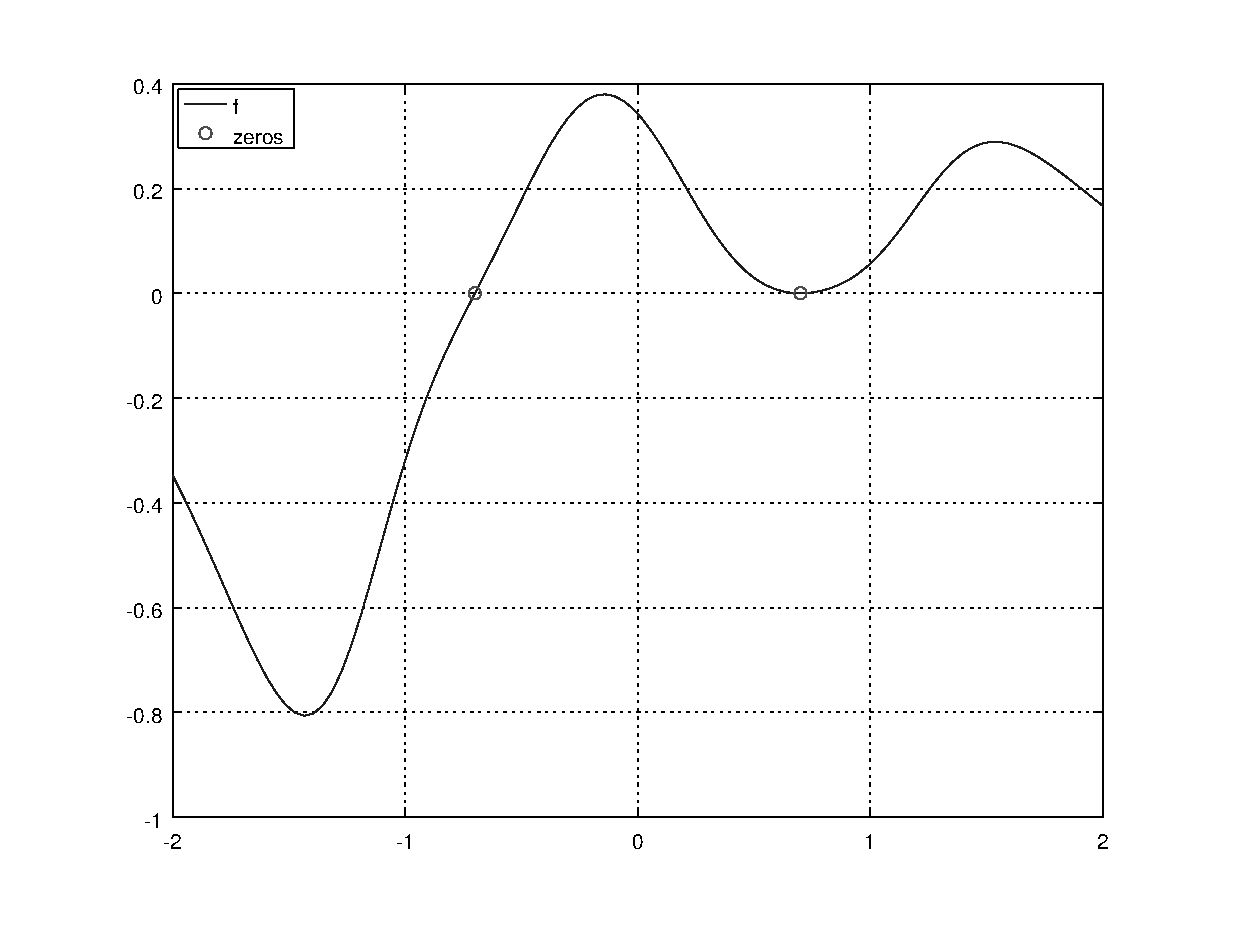
\includegraphics[width=0.8\textwidth]{./cap_eq1d/dados/ex_bis_intro/fig_bis_intro}
  \caption{Esboço da função $f$ do Exemplo~\ref{ex:bis_intro}.}
  \label{fig:bis_intro}
\end{figure}

Observamos que esta função é contínua e que, por exemplo, $f(-2)>0$ e $f(3)<0$, logo $f(-2)\cdot f(3) < 0$ e, de fato, $f$ tem pelo menos um zero\footnote{De fato, $f$ tem três zeros no intervalo $(-2, 3)$.} no intervalo $(-2, 3)$.

\ifisoctave
O esboço do gráfico da função $f$ pode ser feito no \verb+GNU Octave+ com o seguinte \href{https://github.com/phkonzen/notas/blob/master/src/MatematicaNumerica/cap_eq1d/dados/ex_bis_intro/ex_bis_intro.m}{código}:
\verbatiminput{./cap_eq1d/dados/ex_bis_intro/ex_bis_intro.m}
\fi
\end{ex}

Consideremos, então, uma função $f$ contínua tal que $f(a)\cdot f(b) < 0$. O método da bisseção é iterativo, sendo que a primeira aproximação para uma solução de $f(x)=0$ tomada como o ponto médio do intervalo $(a, b)$, i.e.
\begin{equation}
  x^{(1)} = \frac{a^{(1)}+b^{(1)}}{2},
\end{equation}
onde $a^{(1)} = a$ e $b^{(1)} = b$. Daí, se ocorrer $f(x^{(1)})=0$ o problema está resolvido. Caso contrário, $f$ tem pelo menos um zero num dos subintervalos $(a^{(1)}, x^{(1)})$ ou $(x^{(1)}, b^{(1)})$, pois $f(a^{(1)})\cdot f(x^{(1)}) < 0$ ou  $f(x^{(1)})\cdot f(b^{(1)}) < 0$, respectivamente e exclusivamente. No primeiro caso, escolhemos $(a^{(2)}, b^{(2)}) = (a^{(1)}, x^{(1)})$ ou, no segundo caso, tomamos $(a^{(2)}, b^{(2)}) = (x^{(1)}, b^{(1)})$. Então, a segunda aproximação para uma solução é computada como
\begin{equation}
  x^{(2)} = \frac{a^{(2)} + b^{(2)}}{2}.
\end{equation}
Daí, o procedimento se repete até obtermos uma aproximação com a precisão desejada.

\begin{ex}\label{ex:bis_exec}
  Consideremos o problema de encontrar um zero da função
\begin{equation}
  f(x) = \sen^2\left(x+\frac{\pi}{4}\right) - x^3 + \frac{\pi}{4}x^2 + \frac{5\pi^2}{16}x + \frac{3\pi^3}{64}.
\end{equation}
Do esboço de seu gráfico (Figura \ref{fig:bis_intro}) vemos que $f(2)\cdot f(3) \neq 0$ sendo que o zero $x=3\pi/4\approx 2,3562$ de $f$ está no intervalo $(2, 3)$. Então, aplicando o método da bisseção com intervalo inicial $(a^{(1)}, b^{(1)}) = (2, 3)$ e aproximação inicial $x^{(1}) = (a^{(1)}+b^{(1)})/2$, obtemos as aproximações apresentadas na Tabela \ref{tab:bis_exec}.

\begin{table}[h!]
  \centering
  \caption{Resultados referentes ao Exemplo~\ref{ex:bis_exec}.}
  \begin{tabular}{r|rr|r|c}
    k & $a^{(k)}$ & $b^{(k)}$ & $x^{(k)}$ & $f(a^{(k)})\cdot f(x^{(k)})$\\\hline
    1 & $2,0000$ & $3,0000$ & $2,5000$ & -1 \\
    2 & $2,0000$ & $2,5000$ & $2,2500$ &  1 \\
    3 & $2,2500$ & $2,5000$ & $2,3750$ & -1 \\
    4 & $2,2500$ & $2,3750$ & $2,3125$ & 1 \\
    5 & $2,3125$ & $2,3750$ & $2,3438$ & 1 \\
    6 & $2,3438$ & $2,3750$ & $2,3594$ &  -1 \\
    7 & $2,3438$ & $2,3594$ & $2,3516$ & 1 \\
    8 & $2,3516$ & $2,3594$ & $2,3555$ &  1 \\
    9 & $2,3555$ & $2,3594$ & $2,3574$ &  -1 \\
    10 & $2,3555$ & $2,3574$ & $2,3564$ & -1 \\\hline
  \end{tabular}
  \label{tab:bis_exec}
\end{table}

\ifisoctave
A tabela \ref{tab:bis_exec} pode ser obtida no \verb+GNU Octave+ com o seguinte \href{https://github.com/phkonzen/notas/blob/master/src/MatematicaNumerica/cap_eq1d/dados/ex_bis_exec/ex_bis_exec.m}{código}:
\verbatiminput{./cap_eq1d/dados/ex_bis_exec/ex_bis_exec.m}
\fi
\end{ex}

\subsection{Análise de convergência}

Dada uma função estritamente monótona\footnote{Estritamente crescente ou estritamente decrescente.} e contínua $f:[a, b]\to\mathbb{R}$ com $f(a)\cdot f(b) < 0$, temos que o método da bisseção converge para o zero de $f$ no intervalo $(a, b)$. 

De fato, como consequência imediata do \href{https://phkonzen.github.io/notas/AnaliseMatematicaI/cap_continuidade_sec_prop_f_cont.html}{teorema do valor intermediário}, temos que $f$ tem pelo menos um zero no intervalo $(a, b)$. Agora, da hipótese de monotonicidade estrita, temos que $f$ tem um único zero neste intervalo, o qual denotaremos por $x^{*}$.

Da construção das iteradas do método, temos
\begin{align}
  |x^{(k)} - x^{*}| &\leq \frac{b^{(k)}-a^{(k)}}{2}\\
  &\leq \frac{b^{(k-1)}-a^{(k-1)}}{2^2}\\
  &\vdots \\
  &\leq \frac{b^{(1)}-a^{(1)}}{2^k},
\end{align}
donde, temos a seguinte estimativa do erro de truncamento
\begin{equation}\label{eq:bis_est_trunc}
  |x^{(k)} - x^{*}| \leq \frac{b^{(1)}-a^{(1)}}{2^k}.
\end{equation}
E, daí também, segue a convergência do método da bisseção, pois
\begin{equation}
  \lim_{k\to\infty} |x^{(k)}-x^{*}| = \lim_{k\to\infty} \frac{b^{(1)}-a^{(1)}}{2^k} = 0.
\end{equation}

\begin{obs}
  No caso de $f$ não ser estritamente monótona no intervalo $(a, b)$, ainda podemos garantir a convergência do método da bisseção. Isto segue do fato de que após algumas iteradas, digamos $k$ iteradas, a função $f$ terá apenas um zero no intervalo $(a^{(k)}, b^{(k)})$. A partir daí, as estimativas acima podem ser aplicadas.
\end{obs}

\begin{ex}\label{ex:bis_conv}
  No Exemplo \ref{ex:bis_exec} aplicamos o método da bisseção para a função
\begin{equation}
  f(x) = \sen^2\left(x+\frac{\pi}{4}\right) - x^3 + \frac{\pi}{4}x^2 + \frac{5\pi^2}{16}x + \frac{3\pi^3}{64}.
\end{equation}
no intervalo $(2, 3)$. Observando os resultados mostrados na Tabela \ref{tab:bis_exec}, vemos que
\begin{equation}
  |x^{(10)}-x^*| = 2,5\E-4,
\end{equation}
com $x^* = x_1 = 3\pi/4$. Observamos que este resultado é consistente com a estimativa do erro de truncamento \eqref{eq:bis_est_trunc}, da qual temos
\begin{align}
  |x^{(10)} - x^*| &\leq \frac{b^{(1)}-a^{(1)}}{2^{10}}\\
  &= \frac{1}{2^{10}} = 9,8\E-4.
\end{align}
\end{ex}

\begin{obs}(\normalfont{Taxa de convergência.})
  A estimativa de convergência \eqref{eq:bis_est_trunc} também pode ser usada para mostrarmos que, assintoticamente, o método da bisseção tem a seguinte taxa de convergência linear
  \begin{equation}
    \left|x^{(k+1)} - x^{(k)}\right| \lesssim \frac{1}{2}\left|x^{(k)} - x^{(k-1)}\right|^{\pmb{1}}.
  \end{equation}
\end{obs}

\subsection{Zeros múltiplos}

Sejam $f$ uma função suave e $x^*$ um zero de multiplicidade par de $f$. Observamos que o método da bisseção não é diretamente aplicável para aproximar $x^*$. Isto ocorre, pois, neste caso, $x^*$ será um ponto de mínimo ou de máximo local de $f$, não havendo pontos $a$ e $b$ próximos de $x^*$ tal que $f(a)\cdot f(b) < 0$.

Agora, sendo $x^*$ é um zero de multiplicidade $2m$ de $f$, temos que ela admite a seguinte decomposição
\begin{equation}
  f(x) = (x-x^*)^{2m}g(x),
\end{equation}
onde $g$ é uma função suave e $g(x^*)\neq 0$. Daí, a derivada de $f$
\begin{equation}
  f'(x) = 2m(x-x^*)^{2m-1}g(x) + (x-x^*)^{2m}g'(x),
\end{equation}
tem $x^*$ como um zero de multiplicidade $2m-1$ (ímpar) e, desta forma, podemos aplicar o método da bisseção em $f'$ para aproximar $x^*$.

\begin{ex}\label{ex:bis_multpar}
  A função
\begin{equation}
  f(x) = \sen^2\left(x+\frac{\pi}{4}\right) - x^3 + \frac{\pi}{4}x^2 + \frac{5\pi^2}{16}x + \frac{3\pi^3}{64}.
\end{equation}
tem $x=-\pi/4\approx -0,7854$ como um zero de multiplicidade par (veja Figura \ref{fig:bis_intro}). Para aplicarmos o método da bisseção para aproximarmos este zero, primeiramente, derivamos $f$
\begin{equation}
  f'(x) = 2\sin(x+\pi/4)\cos(x+\pi/4) - 3x^2 + \frac{\pi}{2}x + \frac{5\pi^2}{16}.
\end{equation}
O esboço do gráfico de $f'$ (Figura \ref{fig:bis_multpar}) mostra que $f'(-1)\cdot f'(0) < 0$ sendo que no intervalo $(-1, 0)$ $f'$ tem um zero de multiplicidade ímpar. Então, aplicando o método da bisseção a $f'$ no intervalo inicial $(a^{(1)}, b^{(1)}) = (-1, ~0)$, obtemos os resultados apresentados na Tabela~\ref{tab:bis_multpar}. Nesta tabela são apresentados as iteradas até a convergência da solução com precisão de $10^{-3}$.

\begin{figure}[h!]
  \centering
  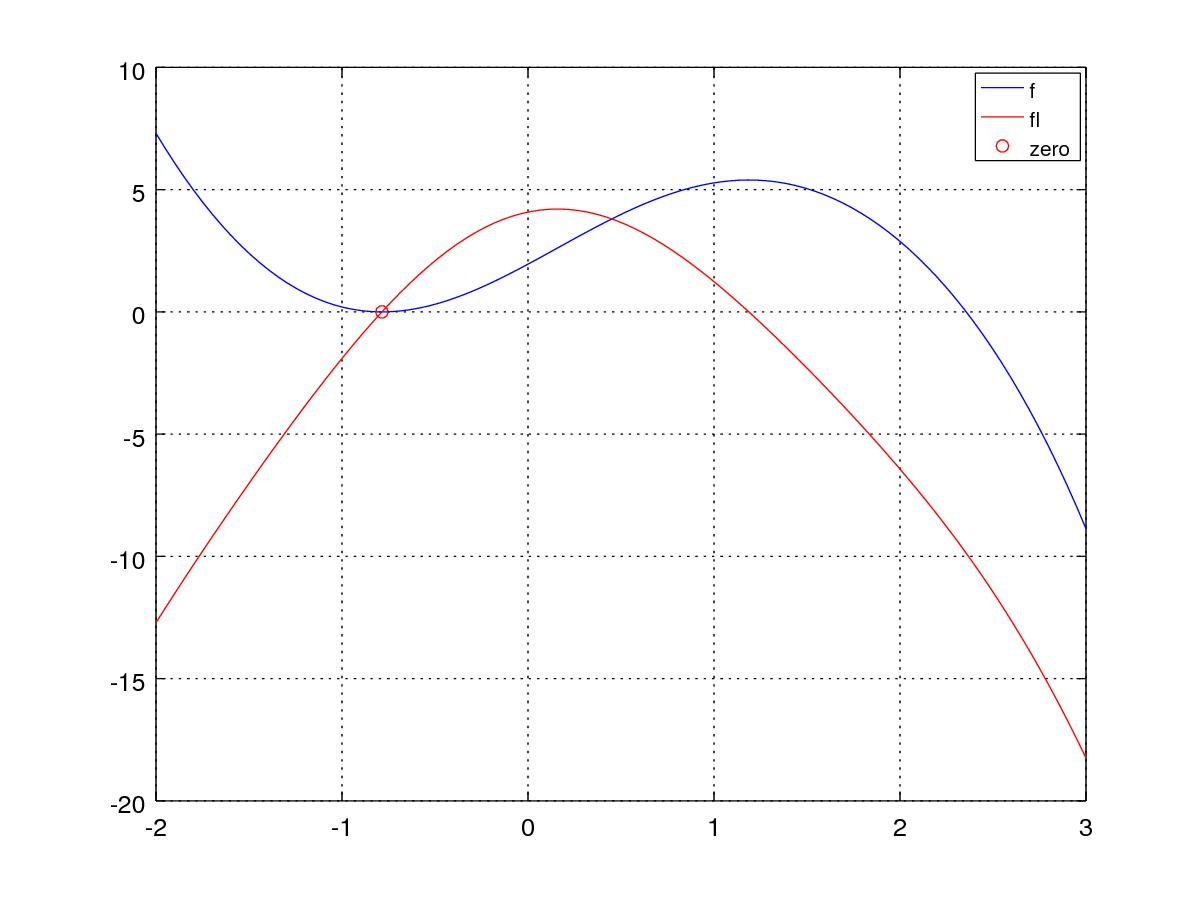
\includegraphics[width=0.8\textwidth]{./cap_eq1d/dados/ex_bis_multpar/fig_bis_multpar}
  \caption{Esboço do gráfico da $f$ e de sua derivada $f'$ dada no Exemplo \ref{ex:bis_multpar}.}
  \label{fig:bis_multpar}
\end{figure}

\begin{table}[h!]
  \centering
  \caption{Resultados referentes ao Exemplo~\ref{ex:bis_exec}.}
  \begin{tabular}{r|rr|r|c}
    k & $a^{(k)}$ & $b^{(k)}$ & $x^{(k)}$ & $f'(a^{(k)})\cdot f'(x^{(k)})$\\\hline
    1 & $-1,0000\E+0$ & $0,0000\E+0$ & $-5,0000\E-1$ & -1 \\
    2 & $-1,0000\E+0$ & $-5,0000\E-1$ & $-7,5000\E-1$ & -1 \\
    3 & $-1,0000\E+0$ & $-7,5000\E-1$ & $-8,7500\E-1$ & 1 \\
    4 & $-8,7500\E-1$ & $-7,5000\E-1$ & $-8,1250\E-1$ &  1 \\
    5 & $-8,1250\E-1$ & $-7,5000\E-1$ & $-7,8125\E-1$ & -1 \\
    6 & $-8,1250\E-1$ & $-7,8125\E-1$ & $-7,9688\E-1$ & 1 \\
    7 & $-7,9688\E-1$ & $-7,8125\E-1$ & $-7,8906\E-1$ & 1 \\
    8 & $-7,8906\E-1$ & $-7,8125\E-1$ & $-7,8516\E-1$ & -1 \\
    9 & $-7,8906\E-1$ & $-7,8516\E-1$ & $-7,8711\E-1$ & 1 \\
    10 & $-7,8711\E-1$ & $-7,8516\E-1$ & $-7,8613\E-1$ & 1 \\\hline
  \end{tabular}
  \label{tab:bis_multpar}
\end{table}

\ifisoctave
A tabela \ref{tab:bis_multpar} pode ser obtida no \verb+GNU Octave+ com o seguinte \href{https://github.com/phkonzen/notas/blob/master/src/MatematicaNumerica/cap_eq1d/dados/ex_bis_multpar/ex_bis_multpar.m}{código}:
\verbatiminput{./cap_eq1d/dados/ex_bis_multpar/ex_bis_multpar.m}
\fi
\end{ex}

\subsection*{Exercícios}

\begin{exer}\label{exer:bis_1}
  Use o método da bisseção para aproximar um zero de $f(x)=x^3\sen(x)-\cos(x)$, aplicando como intervalo inicial $(a^{(1)}, b^{(1)}) = (0,5, ~1)$ e aproximação inicial $x^{(1)}=(a^{(1)}+b^{(1)})/2$. Faça, então, $6$ iterações de forma a obter a aproximação $x^{(7)}$ e forneça-a com $7$ dígitos significativos por arredondamento.
\end{exer}
\begin{resp}
    \ifisoctave 
  \href{https://github.com/phkonzen/notas/blob/master/src/MatematicaNumerica/cap_eq1d/dados/exer_bis_1/exer_bis_1.m}{Código.} 
  \fi
  $9,179688\times 10^{-1}$
\end{resp}

\begin{exer}\label{exer:bis_est_trunc}
  Considere que o método da bisseção para aproximar um zero de $f(x)=x^3\sen(x)-\cos(x)$, aplicando como intervalo inicial $(a^{(1)}, b^{(1)}) = (0,5, ~1)$ e aproximação inicial $x^{(1)}=(a^{(1)}+b^{(1)})/2$. Use a estimativa de convergência \eqref{eq:bis_est_trunc}
  \begin{equation}
    \left|x^{(k)} - x^{*}\right| \leq \frac{b^{(1)}-a^{(1)}}{2^k},
  \end{equation}
para estimar o número mínimo de iterações $k_{conv}$ necessárias para se obter a solução com exatidão de $10^{-4}$. Então, compute $x^{(k_{conv})}$ e forneça-o com $6$ dígitos significativos por arredondamento.
\end{exer}
\begin{resp}
    \ifisoctave 
  \href{https://github.com/phkonzen/notas/blob/master/src/MatematicaNumerica/cap_eq1d/dados/exer_bis_este_trunc/exer_bis_est_trunc.m}{Código.} 
  \fi
  $9,15833\E-1$
\end{resp}

\begin{exer}\label{exer:bis_multpar}
  Use o método da bisseção para encontrar uma aproximação com precisão de $10^{-4}$ do zero de
  \begin{equation}
    f(x) = (-x^2+1,154x-0,332929)\cos(x) + x^2 - 1,154x + 0,332929
  \end{equation}
no intervalo $(0,55, ~0,65)$. Forneça a aproximação computada com $7$ dígitos significativos por arredondamento.
\end{exer}
\begin{resp}
    \ifisoctave 
  \href{https://github.com/phkonzen/notas/blob/master/src/MatematicaNumerica/cap_eq1d/dados/exer_bis_multpar/exer_bis_multpar.m}{Código.} 
  \fi
  $5,770508\times 10^{-1}$
\end{resp}

\section{Método da falsa posição}\label{cap_eq1d_sec_falsapos}

O método da falsa posição é uma variação do método da bisseção. Dada uma função $f$ contínua, escolhemos um intervalo inicial $(a, b)$ tal que $f(a)\cdot f(b) < 0$ (i.e. $f$ tem sinais trocados nos pontos $a$ e $b$). Então, uma aproximação para o zero de $f$ neste intervalo é computada como o ponto de interseção da reta secante a $f$ pelos pontos $(a, f(a))$ e $(b, f(b))$, i.e.
\begin{equation}
  x = a - \frac{b-a}{f(b)-f(a)}f(a).
\end{equation}
Veja a Figura \ref{fig:falsapos}.

\begin{figure}[h!]
  \centering
  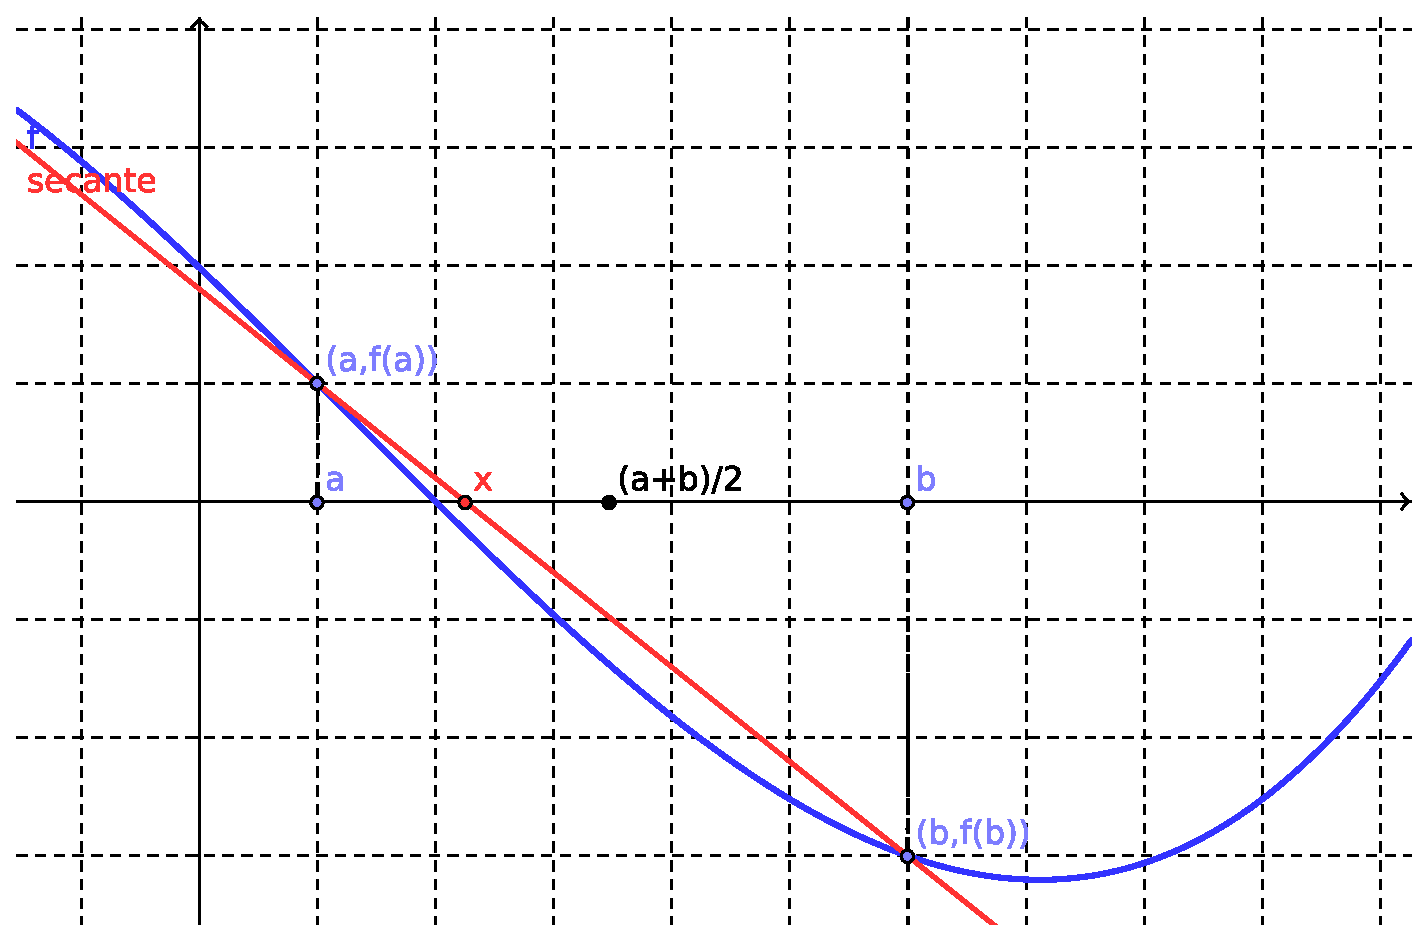
\includegraphics[width=0.7\textwidth]{./cap_eq1d/dados/fig_falsapos/fig_falsapos}
  \caption{Ilustração do método da falsa posição (veja no \href{https://github.com/phkonzen/notas/blob/master/src/MatematicaNumerica/cap_eq1d/dados/fig_falsapos/fig_falsapos.ggb}{Geogebra}).}
  \label{fig:falsapos}
\end{figure}

Mais explicitamente, o método da falsa posição consiste no seguinte procedimento iterativo:
\begin{enumerate}
\item Determinar um intervalo $(a^{(1)}, b^{(1)})$ tal que $f(a^{(1)})\cdot f(b^{(1)}) \neq 0$.
\item Para $k = 1, 2, 3, \cdots, N$:
  \begin{enumerate}[2.1]
  \item $\displaystyle x^{(k)} = a^{(k)} - \frac{b^{(k)}-a^{(k)}}{f(b^{(k)})-f(a^{(k)})}f(a^{(k)})$
  \item Verificar critério de parada.
  \item Se $f(a^{(k)})\cdot f(x^{(k)}) \neq 0$, então $a^{(k+1)}=a^{(k)}$ e $b^{(k+1)}=x^{(k)}$.
  \item Se $f(x^{(k)})\cdot f(b^{(k)}) \neq 0$, então $a^{(k+1)}=x^{(k)}$ e $b^{(k+1)}=b^{(k)}$.
  \end{enumerate}
\end{enumerate}

\begin{ex}\label{ex:falsapos_exec}
  Consideremos o problema de aproximar o zero de
\begin{equation}
  f(x) = \sen^2\left(x+\frac{\pi}{4}\right) - x^3 + \frac{\pi}{4}x^2 + \frac{5\pi^2}{16}x + \frac{3\pi^3}{64}.
\end{equation}
no intervalo $(0, 3)$. A Tabela \ref{tab:falsapos_exec} mostra os resultados obtidos da aplicação do método da falsa posição com intervalo inicial $(a^{(1)}, b^{(1)}) = (2, 3)$. Aqui, o método foi iterado até a convergência com cinco dígitos significativos.

\begin{table}[h!]
  \centering
  \caption{Resultados referentes ao Exemplo~\ref{ex:falsapos_exec}.}
  \begin{tabular}{r|rr|r|c}
    k & $a^{(k)}$ & $b^{(k)}$ & $x^{(k)}$ & $f'(a^{(k)})\cdot f'(x^{(k)})$\\\hline
    1 & $2,0000$ & $3,0000$ & $2,2455$ & 1 \\
    2 & $2,2455$ & $3,0000$ & $2,3240$ &  1 \\
    3 & $2,3240$ & $3,0000$ & $2,3470$ & 1 \\
    4 & $2,3470$ & $3,0000$ & $2,3536$ & 1 \\
    5 & $2,3536$ & $3,0000$ & $2,3555$ & 1 \\
    6 & $2,3555$ & $3,0000$ & $2,3560$ & 1 \\
    7 & $2,3560$ & $3,0000$ & $2,3561$ &  1 \\
    8 & $2,3561$ & $3,0000$ & $2,3562$ & 1 \\
    9 & $2,3562$ & $3,0000$ & $2,3562$ & 1 \\
    10 & $2,3562$ & $3,0000$ & $2,3562$ & 1 \\\hline
  \end{tabular}
  \label{tab:falsapos_exec}
\end{table}

\ifisoctave
A tabela \ref{tab:falsapos_exec} pode ser obtida no \verb+GNU Octave+ com o seguinte \href{https://github.com/phkonzen/notas/blob/master/src/MatematicaNumerica/cap_eq1d/dados/ex_falsapos_exec/ex_falsapos_exec.m}{código}:
\verbatiminput{./cap_eq1d/dados/ex_falsapos_exec/ex_falsapos_exec.m}
\fi
\end{ex}

\subsection*{Exercícios}

\begin{exer}\label{exer:falsapos_1}
  Use o método da falsa posição para aproximar um zero de $f(x)=x^3\sen(x)-\cos(x)$, aplicando como intervalo inicial $(a^{(1)}, b^{(1)}) = (0,5, ~1)$ e aproximação inicial
  \begin{equation}
    x^{(1)} = a^{(1)} - \frac{b^{(1)}-a^{(1)}}{f(b^{(1)})-f(a^{(1)})}f(a^{(1)}).
  \end{equation}
Faça, então, $4$ iterações deste método de forma a obter a aproximação $x^{(5)}$ e forneça-a com $7$ dígitos significativos por arredondamento.
\end{exer}
\begin{resp}
    \ifisoctave 
  \href{https://github.com/phkonzen/notas/blob/master/src/MatematicaNumerica/cap_eq1d/dados/exer_falsapos_1/exer_falsapos_1.m}{Código.} 
  \fi
  $9,158079\times 10^{-1}$
\end{resp}

\begin{exer}\label{exer:falsapos_multpar}
  Use o método da bisseção para encontrar uma aproximação com precisão de $10^{-4}$ do zero de
  \begin{equation}
    f(x) = (-x^2+1,154x-0,332929)\cos(x) + x^2 - 1,154x + 0,332929
  \end{equation}
no intervalo $(0,55, ~0,65)$. Forneça a aproximação computada com $7$ dígitos significativos por arredondamento.
\end{exer}
\begin{resp}
    \ifisoctave 
  \href{https://github.com/phkonzen/notas/blob/master/src/MatematicaNumerica/cap_eq1d/dados/exer_falsapos_multpar/exer_falsapos_multpar.m}{Código.} 
  \fi
  $5,76984\times 10^{-1}$
\end{resp}

\section{Iteração de ponto fixo}\label{cap_eq1d_pfixo}

O ponto fixo de uma função dada $g$ é o ponto $x$ tal que
\begin{equation}
  g(x) = x.
\end{equation}
Geometricamente, pontos fixos são interseções do gráfico da $g$ com a reta $y=x$, veja a Figura \ref{fig:pfixo}.

\begin{figure}[h!]
  \centering
  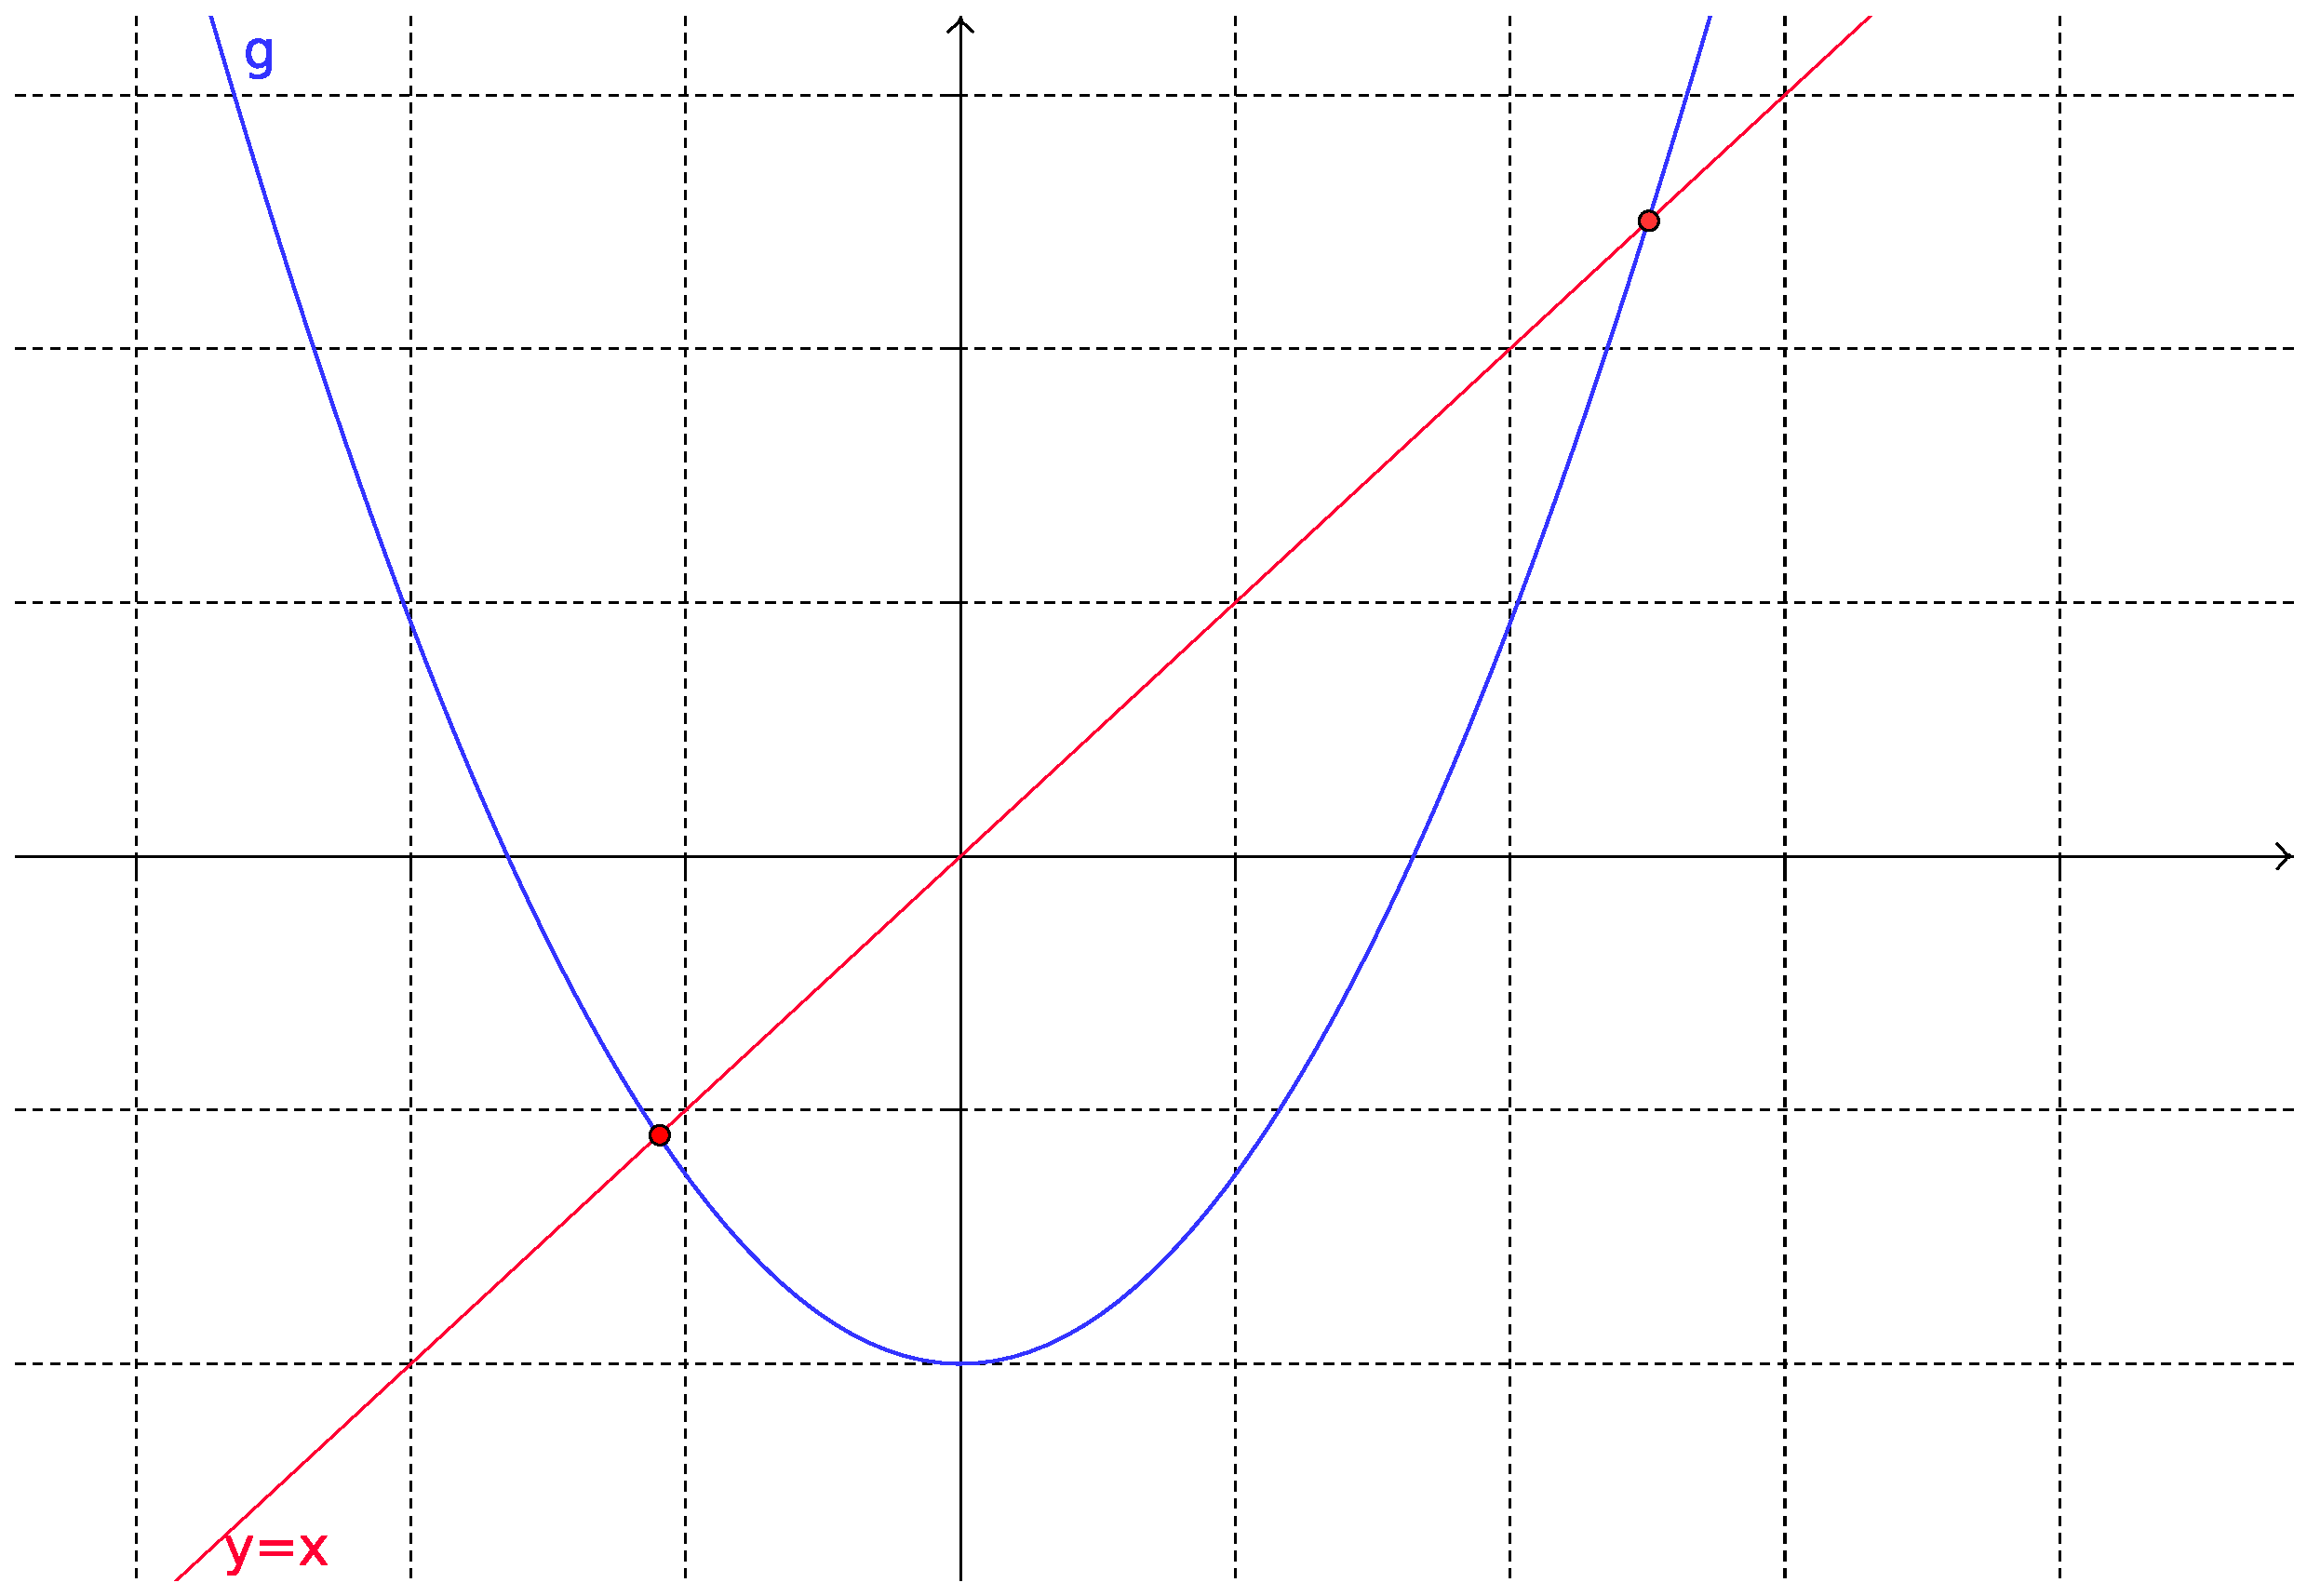
\includegraphics[width=0.8\textwidth]{./cap_eq1d/dados/fig_pfixo/fig_pfixo}
  \caption{Exemplos de pontos fixos (veja no \href{https://github.com/phkonzen/notas/blob/master/src/MatematicaNumerica/cap_eq1d/dados/fig_pfixo/fig_pfixo.ggb}{Geogebra}).}
  \label{fig:pfixo}
\end{figure}

Observamos que toda equação de uma incógnita pode ser reescrita de forma equivalente como um problema de ponto fixo.

\begin{ex}\label{ex:pfixo_intro}
  Consideremos o problema de resolver
  \begin{equation}
    \sen^2\left(x+\frac{\pi}{4}\right) = x^3 - \frac{\pi}{4}x^2 - \frac{5\pi^2}{16}x - \frac{3\pi^3}{64}.
  \end{equation}
Podemos reescrevê-la como o problema de se obter os zeros da seguinte função
\begin{equation}
  f(x) = \sen^2\left(x+\frac{\pi}{4}\right) - x^3 + \frac{\pi}{4}x^2 + \frac{5\pi^2}{16}x + \frac{3\pi^3}{64}.
\end{equation}
Por sua vez, este problema é equivalente aos seguintes problemas de ponto fixo (entre outros):
\begin{align}
  &a)~g_1(x) = \frac{16}{5\pi^2}\left[-\sen^2\left(x+\frac{\pi}{4}\right) + x^3 - \frac{\pi}{4}x^2 - \frac{3\pi^3}{64}\right] = x.\\
  &b)~g_2(x) = \sqrt[3]{\sen^2\left(x+\frac{\pi}{4}\right) + \frac{\pi}{4}x^2 + \frac{5\pi^2}{16}x + \frac{3\pi^3}{64}}
\end{align}
Na Figura \ref{fig:pfixo_intro} podemos observar que os zeros da $f$ (a saber, $x_1=3\pi/4\approx 2,3562$ e $x_2=x_3=-\pi/4\approx -0,78540$) coincidem com os pontos fixos das funções $g_1$ e $g_2$.

\begin{figure}[h!]
  \centering
  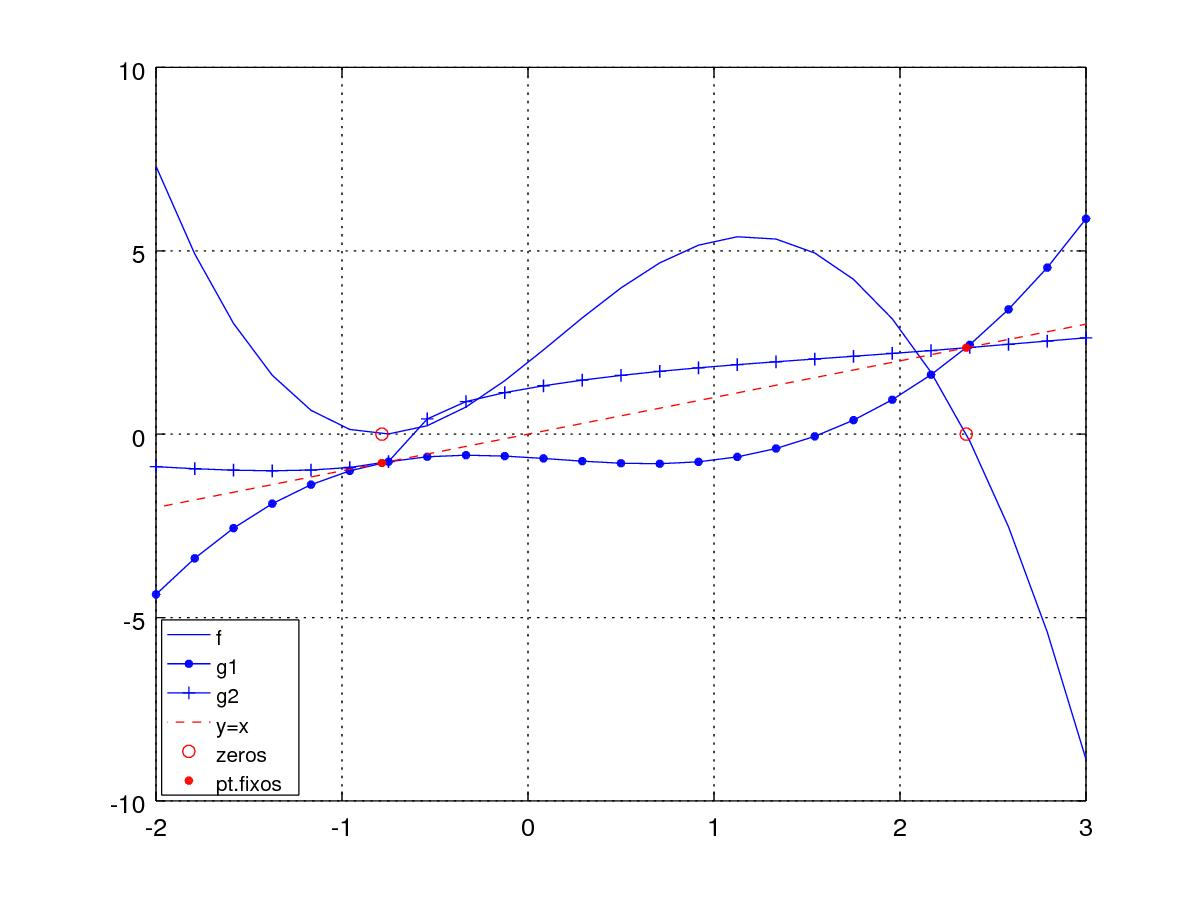
\includegraphics[width=0.8\textwidth]{./cap_eq1d/dados/ex_pfixo_intro/fig_pfixo_intro}
  \caption{Esboço da função $f$ do Exemplo~\ref{ex:pfixo_intro}.}
  \label{fig:pfixo_intro}
\end{figure}
\end{ex}

Em muitos casos, é possível obter aproximações de um ponto fixo de uma dada função $g$ pela chamada \emph{iteração de ponto fixo}:
\begin{align}
  x^{(1)} &= \text{aprox. inicial}\\
  x^{(k+1)} = g(x^{(k)}),\quad k=1, 2, 3, \ldots
\end{align}

\begin{ex}\label{ex:pfixo_testes}
  Observemos que para a função $g_1$ dada no Exemplo \ref{ex:pfixo_intro}, temos as seguintes iterações:
  \begin{align}
    x^{(1)} &= -0,70000,\\
    x^{(2)} &= -0,70959,\\
    x^{(3)} &= -0,71716,\\
    &\vdots \\
    x^{(100)} &= -0,77862,\\
    &\vdots \\
    x^{(1000)} &= -0,78466,\\    
    &\vdots \\
    x^{(20000)} &= -0,78536.
  \end{align}
Ou seja, neste caso as iterações de ponto fixo convergem (lentamente) para o ponto fixo $x=-\pi/4\approx -0,78540$.
\ifisoctave
Veja o \href{https://github.com/phkonzen/notas/blob/master/src/MatematicaNumerica/cap_eq1d/dados/ex_pfixo_testes/ex_g1_t1.m}{código} no \verb+GNU Octave+.
\fi

Agora, se usarmos a iteração de ponto fixo com esta mesma função para aproximar o ponto fixo $x=3\pi/4\approx 2,3562$, obtemos
  \begin{align}
    x^{(1)} &= 2,50000,\\
    x^{(2)} &= 2,9966,\\
    x^{(3)} &= 5,8509,\\
    &\vdots \\
    x^{(8)} &= 4,8921e\times 10^{121}.
  \end{align}
Donde observamos que as iterações divergem rapidamente.

Entretanto, se usarmos a iteração de ponto fixo com a função $f_2$ dada no Exemplo \ref{ex:pfixo_intro}, obtemos
  \begin{align}
    x^{(1)} &= 2,50000,\\
    x^{(2)} &= 2,4155,\\
    x^{(3)} &= 2,3805,\\
    &\vdots \\
    x^{(10)} &= 2,3562.
  \end{align}
A qual, portanto, converge para o ponto fixo esperado.
\end{ex}

Este último exemplo (Exemplo \ref{ex:pfixo_testes}) mostra que a iteração do ponto fixo nem sempre é convergente. Por sorte, o seguinte teorema nos fornece condições suficientes para a convergência destas iterações.

\begin{teo}(\normalfont{Teorema do ponto fixo})\label{teo:pfixo}
  Seja uma dada função $g$ continuamente diferenciável satisfazendo
  \begin{enumerate}[a)]
  \item $g([a, b]) \subset [a, b]$,
  \item $|g'(x)|<K<1$ para todo $x\in [a, b]$.
  \end{enumerate}
Então, $g$ tem um único ponto fixo $x^*\in [a, b]$ e as iterações $x^{(k+1)}=x^{(k)}$, $k=1, 2, 3, \ldots$, convergem para $x^*$, para qualquer escolha de $x^{(1)}\in [a, b]$.
\end{teo}
\begin{dem}
  Da hipótese b), temos que $g$ é uma contração com
  \begin{equation}
    |g(x) - g(y)| < K\cdot |x - y|,~\forall x,y\in [a, b].
  \end{equation}
Com isso, da hipótese a) e tomando $x^{(1)}\in [a, b]$, temos
\begin{align}
  |x^{(k+1)} - x^{(k)}| &= |g(x^{(k)}) - g(x^{(k-1)})|\\
  &\leq K |x^{(k)} - x^{(k-1)}|\\
  &\vdots \\
  &\leq K^{k-1}|x^{(2)}-x^{(1)}|,
\end{align}
para todo $k=2, 3, \ldots$. Como $K<1$, temos $|x^{(k+1)}-x^{(k)}|\to 0$ quando $k\to\infty$ e, portanto, $x^{(k)}$ converge para algum $x^*\in [a, b]$.

De fato, $x^*$ é ponto fixo de $g$, pois da continuidade da $g$, temos
\begin{equation}
  x^* = \lim_{k\to\infty} x^{(k+1)} = \lim_{k\to\infty} g(x^{(k)}) = g(x^*).
\end{equation}

Por fim, $x^*$ é único, pois assumindo a existência de outro ponto fixo $x^{**}\neq x^*$ teríamos
\begin{equation}
  |x^* - x^{**}| = |g(x^*) - g(x^{**})| < K|x^* - x^{**}|.
\end{equation}
\end{dem}

Agora, dado um problema de encontrar um zero de uma dada função $f$, i.e. $f(x)=0$, podemos construir uma função $g$ para a iteração de ponto fixo associada da seguinte forma:
\begin{align}
  f(x) = 0 &\Leftrightarrow \underbrace{x - \alpha f(x)}_{g(x)} = x,
\end{align}
com $\alpha\in\mathbb{R}$ escolhido de forma a satisfazer as hipóteses do teorema do ponto fixo (Teorema \ref{teo:pfixo}).

\begin{ex}\label{ex:pfixo_exec}
  Retornamos ao problema de encontrar o zero da função
  \begin{equation}
    f(x) = \sen^2\left(x+\frac{\pi}{4}\right) - x^3 + \frac{\pi}{4}x^2 + \frac{5\pi^2}{16}x + \frac{3\pi^3}{64}.
  \end{equation}
  no intervalo $[2,3]$. Para construir uma função $g$ para a iteração de ponto fixo neste intervalo, podemos tomar
  \begin{equation}
    g(x) = x - \alpha f(x),
  \end{equation}
com $\alpha = -0,1$. A Figura \ref{fig:ex_pfixo_exec} mostra esboços dos gráficos de $g$ e $|g'|$ no intervalos $[2, 3]$ e podemos observar que esta escolha de $\alpha$ faz com que a $g$ satisfaça o teorema do ponto fixo.

\begin{figure}[h!]
  \centering
  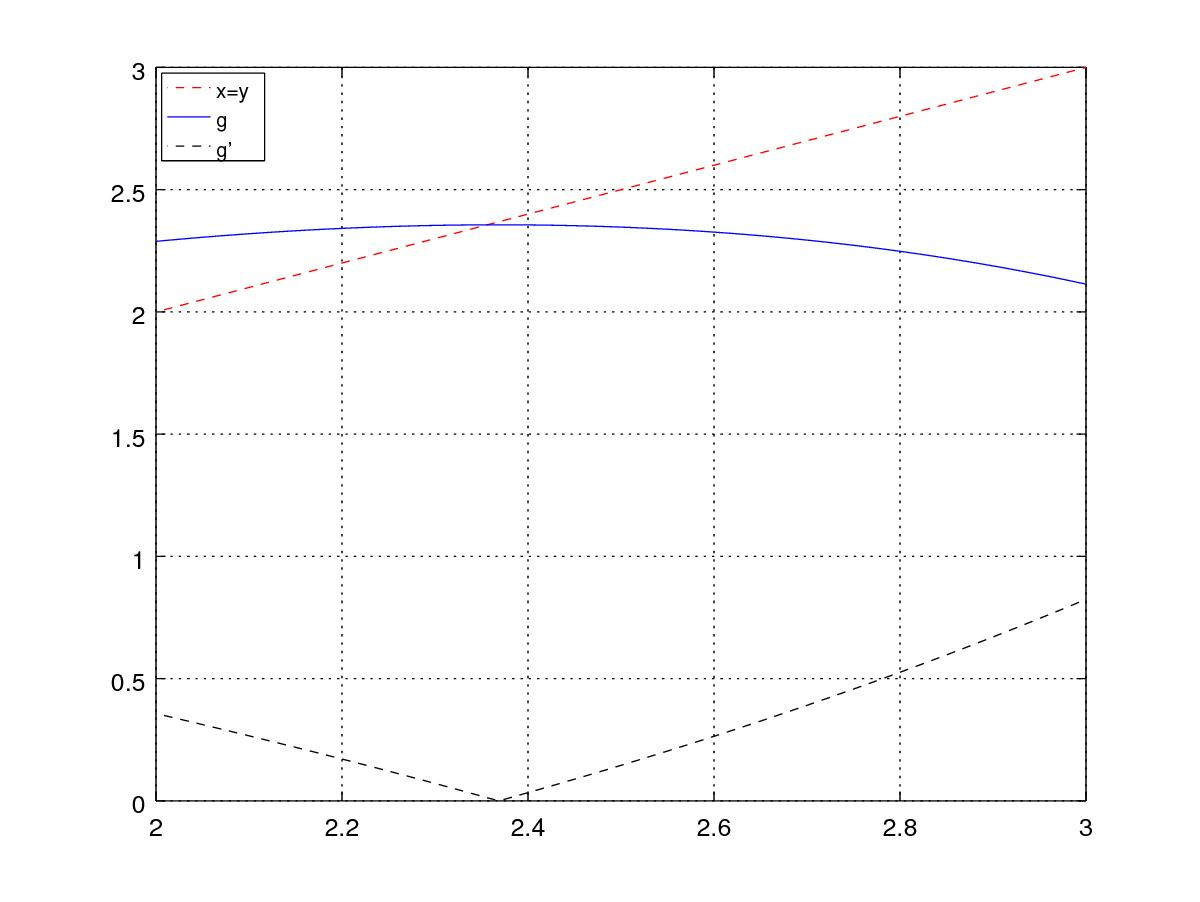
\includegraphics[width=0.8\textwidth]{./cap_eq1d/dados/ex_pfixo_exec/fig_ex_pfixo_exec}
  \caption{Esboço dos gráficos de $g$ e $|g'|$ discutidas no Exemplo \ref{ex:pfixo_exec}.}
  \label{fig:ex_pfixo_exec}
\end{figure}

Então, fazendo as iterações de ponto fixo com aproximação inicial $x^{(1)}=2,6$, obtemos os resultados apresentados na Tabela \ref{tab:ex_pfixo_exec}.

\begin{table}[h!]
  \centering
  \begin{tabular}{r|cc}
    $k$ & $x^{(k)}$ & $|x^{(k)}-x^{(k-1)}|$ \\\hline
    1 & $2,6000$ & -x-\\
    2 & $2,3264$ & $2,7\E-1$ \\
    3 & $2,3553$ & $2,9\E-2$ \\
    4 & $2,3562$ & $8,4\E-4$ \\
    5 & $2,3562$ & $1,1\E-5$ \\\hline
  \end{tabular}
  \caption{Resultados referentes ao Exemplo \ref{ex:pfixo_exec}.}
  \label{tab:ex_pfixo_exec}
\end{table}

\ifisoctave
Os resultados apresentados na Tabela \ref{tab:ex_pfixo_exec} podem ser computados no \verb+GNU Octave+ co o seguinte código:
\verbatiminput{./cap_eq1d/dados/ex_pfixo_exec/ex_pfixo_exec.m}
\fi
\end{ex}

\begin{obs}(\normalfont{Taxa de convergência})
  A iteração de ponto fixo tem taxa de convergência linear
  \begin{equation}
    |x^{(k+1)} - x^{(k)}| < K|x^{(k)} - x^{(k-1)}|^{\pmb{1}},
  \end{equation}
onde $K > 0$ é a constante dada na hipótese $b)$ do teorema do ponto fixo (Teorema \ref{teo:pfixo}). Além disso, isso mostra que quanto menor o valor da constante $K$, mais rápida será a convergência das iterações de ponto fixo.
\end{obs}

\subsection*{Exercícios}

\emconstrucao